% Preamble
\documentclass[12pt]{article}

% Packages
\usepackage{amsmath}
\usepackage{hyperref}
\usepackage[utf8]{inputenc}
\usepackage[T1]{fontenc}
\usepackage{graphicx}
\usepackage{color}
\usepackage{rotating}
\usepackage{float}
\usepackage[format=plain, indention=1cm, scriptsize, font=sf, labelfont=bf]{caption}
\usepackage{chngpage}
\usepackage[inner=3.5cm, outer=3cm, top=3cm, bottom=2cm, includehead, includefoot]{geometry}

\clubpenalty=10000
\widowpenalty=10000

\definecolor{LinkColor}{rgb}{0,0,0.75}

\hypersetup{
	pdftitle = {Zufallszahlentest},
	pdfsubject = {Zufallszahlentest mit dem Spektraltest},
	pdfauthor = {Christian Locatelli, Alexander Wallrodt},
	bookmarksnumbered = true,
	bookmarksopen = false,
	colorlinks = false,
	hypertexnames = true,
	colorlinks=true,
	linkcolor=LinkColor,
	citecolor=LinkColor,
	filecolor=LinkColor,
	menucolor=LinkColor,
	urlcolor=LinkColor,
	breaklinks=true
}

\title{\textbf{Zufallszahlen Spektraltest}}
\author{Christian Locatelli, Alexander Wallrodt}
\date{\today}

% Document
\begin{document}
    % Titelseite
    \maketitle
    \clearpage

    % Inhaltsverzeichnis
    \tableofcontents
    % Liste der Tabellen
    \listoftables
    % Liste der Bilder
    \listoffigures

    \clearpage


    \section{Einleitung}\label{sec:Einleitung}
    In diesem Projekt geht es um die Frage, inwieweit von einem Computer per Algorithmus erzeugte Pseudozufallszahlen
    auch wirklich als zufällig zu Erachten sind.
    Es werden daher insgesamt vier unterschiedliche Zufallszahlengeneratoren mit einem Sprektraltest untersucht und dabei erörtert,
    ob zwischen den erzeugten Zufallszahlen ein kausaler Zusammenhang besteht
    und ob diese Generatoren den Zufall gut simulieren können.

    \section{Die Generatoren}\label{sec:die-generatoren}
    Im Folgenden werden die verwendeten Generatoren beschrieben und erklärt, wie sie funktionieren beziehungsweise wie
    die Zufallszahlen in den einzelnen Generatoren erzeugt werden.

    \subsection{Der LCG}\label{subsec:der-lcg}
    Der LCG ist ein einfacher deterministischer Generator, welcher mit den Startwerten $a$, $x_n$, $c$, $m$ aufgerufen wird.
    $a$ ist der Faktor, $x_n$ der Startwert, $c$ ist das Inkrement und $m$ der Modulus:

    \begin{align*}
    x_{n+1} = (a * x_n + c) \bmod m
    \end{align*}

    \noindent
    Diese können beliebig gewählt werden, jedoch sehen nur mit bestimmten Werten die Zufallsergebnisse auch "zufällig" aus.
    In diesem Projekt wurden die Werte des TI-59 von Texas Instruments gewählt~\cite{lcg}:

    \begin{align*}
    x_{n+1} = (24298 * 0 + 99991) \bmod 199017
    \end{align*}

    \subsection{Die Zufallsgeneratoren von Python}\label{subsec:die-zufallsgeneratoren-von-python}
    Python hat selbst verschiedene Zufallszahlengeneratoren integriert, die Pseudozufallszahlen erstellen können.
    Hierbei wird der sogenannte Mersenne-Twister verwendet.
    Dieser wurde mit der Absicht entwickelt die Schwachstellen der LCGs lösen, unter anderem,
    indem er eine sehr hohe Periode von $p=2^{19937}-1$ besitzt und Floats mit einer Genauigkeit von 53 Bit erzeugt.
    Er gilt als einer der am häufigsten getesteten Zufallsgeneratoren, ist jedoch vollständig deterministisch,
    weswegen er beispielsweise für Kryptografie ungeeignet wäre~\cite{python-random,mersenne-twister}.
    Im Programm werden die Methoden \texttt{random.random()} und \texttt{numpy.random.random()} getestet.

    \vfill

    \subsection{Der Random.org Generator}\label{subsec:der-random.org-generator}
    Random.org ist eine Internetseite, die sich darauf spezialisiert hat, Zufallszahlen zu erzeugen.
    Sie wird unter anderem für Lotterien und Online-Spiele, aber auch für diverse wissenschaftliche
    Anwendungen verwendet.
    Hierbei behaupten die Entwickler, der Generator würde mithilfe von atmosphärischem Rauschen echte Zufallszahlen erstellen,
    die besser sind als die von Computer erstellten Pseudozufallszahlen.
    Die Behauptungen wurden von zwei wissenschaftlichen Untersuchungen bestätigt~\cite{random-org}.

    \vfill

    \section{Durchführung}\label{sec:Durchfuehrung}
    Um die Generatoren auf ihre Zufälligkeit zu überprüfen wurde der Spektraltest verwendet.
    Bei diesem werden Tupel gebildet, welche man als Punkt im mehrdimensionalen Raum interpretiert und darstellt.
    Ziel ist dabei eine gleichmäßig verteilte Menge von Tupeln.
    Wenn sich jedoch Muster erkennen lassen, kann man direkt festhalten, dass ein stochastische Abhängigkeit vorherrscht~\cite{spektraltest}.
    \\
    In diesem Projekt wurden zur Veranschaulichung 2er-Tupel und 3er-Tupel gebildet,
    welche in einem XY-Diagramm beziehungsweise XYZ-Diagramm dargestellt sind.
    \\
    Der Spektraltest wurde dabei auf jeden der vier verschiedenen Generatoren angewandt.
    Um einen guten Vergleich der Generatoren zu ermöglichen, geben alle Generatoren Fließkommazahlen zwischen 0 und 1 zurück.
    Bei jedem Generator wurden 100.000 Zufallszahlen abgerufen, jedoch ist man bei Random.org beschränkt,
    weswegen dort nur 10.000 Zufallszahlen abgerufen wurden.

    \vfill

    \section{Ergebnisse}\label{sec:Ergebnisse}
    Die Ergebnisse sind in einer Tabelle festgehalten.

    \newgeometry{top=1cm, left=1cm, right=1cm}

    \begin{table}

        \centering

        \caption[Ergebnisstabelle]{Ergebnisstabelle}

        \begin{tabular}{|c||c|c|}

            \hline
            & XY-Tupel & XYZ-Tupel \\

            \hline
            \hline

            \rotatebox{90}{LCG} &
            \begin{minipage}[b]{7.5cm}
                \centering
                \captionsetup{font=scriptsize}
                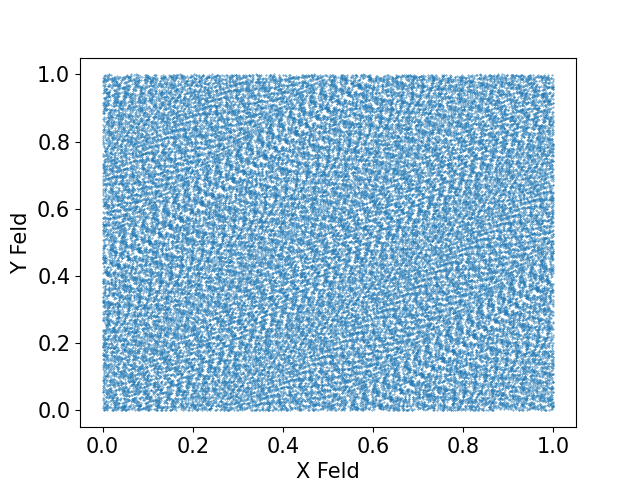
\includegraphics[width=6cm]{images/Random_numbers_by_lcg_with_an_amount_of_100000_numbers_in_2D}
                \captionof{figure}[LCG mit 100000 Zahlen in 2D]{mit 100000 Zahlen}
                \label{fig:figure}
            \end{minipage}
            &
            \begin{minipage}[b]{7.5cm}
                \centering
                \captionsetup{font=scriptsize}
                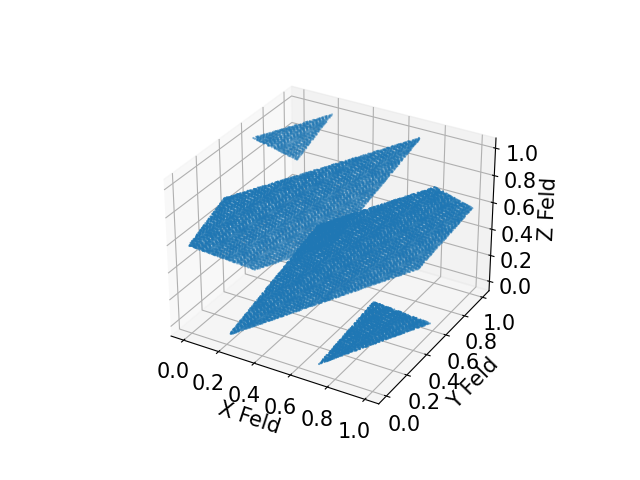
\includegraphics[width=6cm]{images/Random_numbers_by_lcg_with_an_amount_of_100000_numbers_in_3D}
                \captionof{figure}[LCG mit 100000 Zahlen in 3D]{mit 100000 Zahlen}
                \label{fig:figure2}
            \end{minipage}

            \\

            \hline

            \rotatebox{90}{Random Library} &
            \begin{minipage}[b]{7.5cm}
                \centering
                \captionsetup{font=scriptsize}
                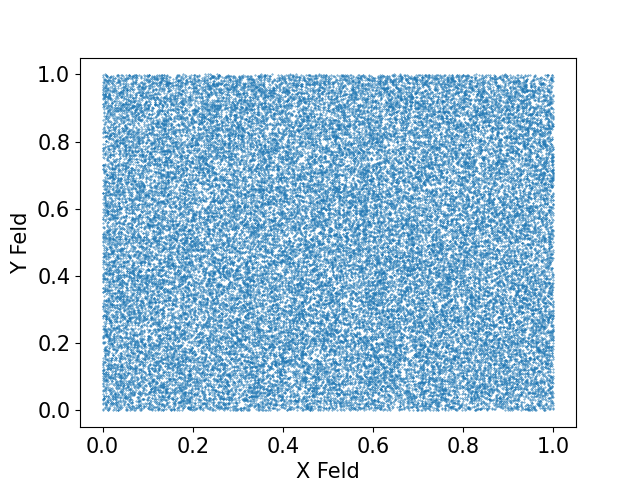
\includegraphics[width=6cm]{images/Random_numbers_by_random_lib_with_an_amount_of_100000_numbers_in_2D}
                \captionof{figure}[Random Library mit 100000 Zahlen in 2D]{mit 100000 Zahlen}
                \label{fig:figure3}
            \end{minipage}
            &
            \begin{minipage}[b]{7.5cm}
                \centering
                \captionsetup{font=scriptsize}
                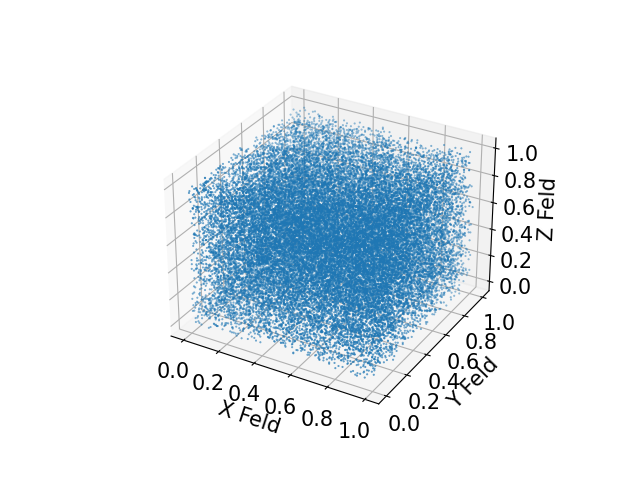
\includegraphics[width=6cm]{images/Random_numbers_by_random_lib_with_an_amount_of_100000_numbers_in_3D}
                \captionof{figure}[Random Library mit 100000 Zahlen in 3D]{mit 100000 Zahlen}
                \label{fig:figure4}
            \end{minipage}

            \\

            \hline

            \rotatebox{90}{Numpy Library} &
            \begin{minipage}[b]{7.5cm}
                \centering
                \captionsetup{font=scriptsize}
                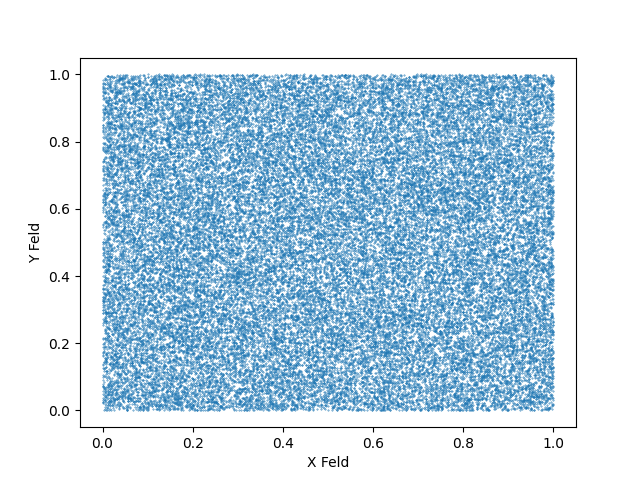
\includegraphics[width=6cm]{images/Random_numbers_by_numpy_lib_with_an_amount_of_100000_numbers_in_2D}
                \captionof{figure}[Numpy Library mit 100000 Zahlen in 2D]{mit 100000 Zahlen}
                \label{fig:figure5}
            \end{minipage}
            &
            \begin{minipage}[b]{7.5cm}
                \centering
                \captionsetup{font=scriptsize}
                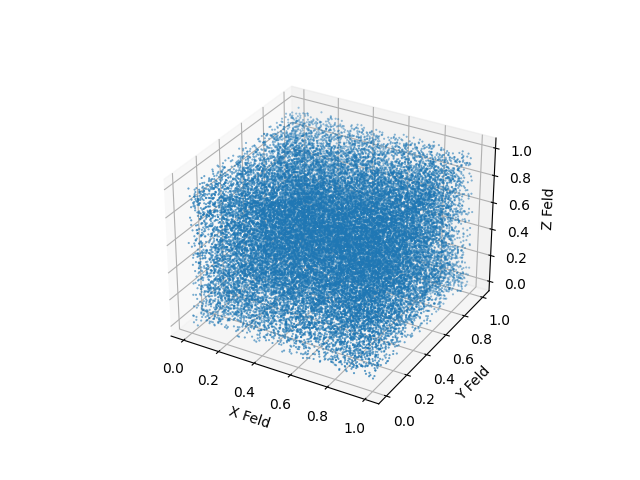
\includegraphics[width=6cm]{images/Random_numbers_by_numpy_lib_with_an_amount_of_100000_numbers_in_3D}
                \captionof{figure}[Numpy Library mit 100000 Zahlen in 3D]{mit 100000 Zahlen}
                \label{fig:figure6}
            \end{minipage}

            \\
            \hline

            \rotatebox{90}{Random.org} &
            \begin{minipage}[b]{7.5cm}
                \centering
                \captionsetup{font=scriptsize}
                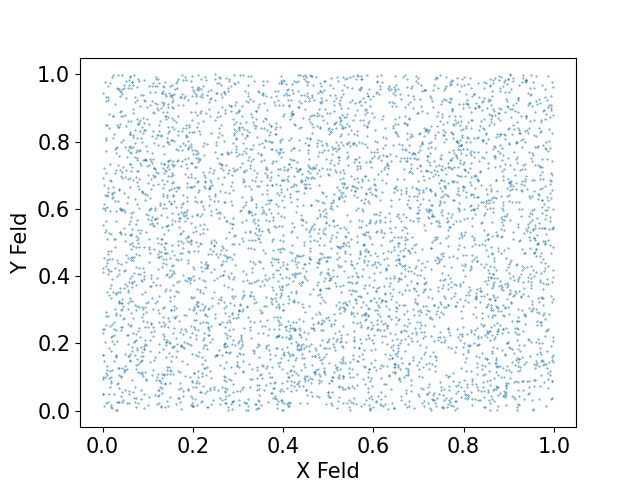
\includegraphics[width=6cm]{images/Random_numbers_by_random_org_with_an_amount_of_10000_numbers_in_2D}
                \captionof{figure}[Random.org mit 100000 Zahlen in 2D]{mit 10000 Zahlen}
                \label{fig:figure7}
            \end{minipage}
            &
            \begin{minipage}[b]{7.5cm}
                \centering
                \captionsetup{font=scriptsize}
                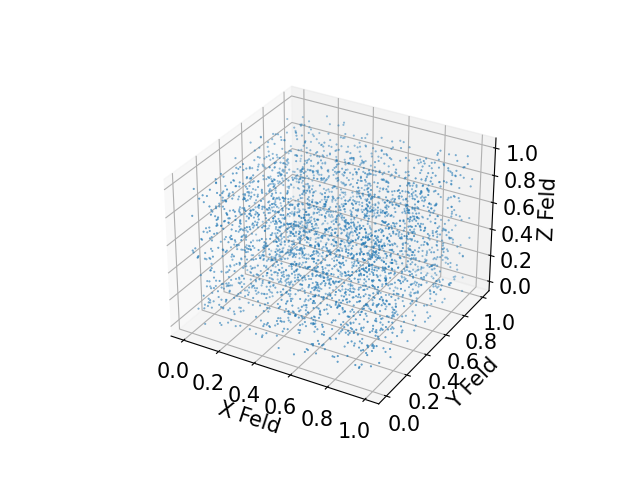
\includegraphics[width=6cm]{images/Random_numbers_by_random_org_with_an_amount_of_10000_numbers_in_3D}
                \captionof{figure}[Random.org mit 100000 Zahlen in 3D]{mit 10000 Zahlen}
                \label{fig:figure8}
            \end{minipage}

            \\

            \hline

        \end{tabular}\label{tab:ergebnisse}

    \end{table}

    \restoregeometry


    \section{Fazit}\label{sec:fazit}
    Die Ergebnisse zeigen, dass der LCG kein guter Generator ist,
    da in der 2D- und 3D-Darstellung Muster zu erkennen sind und somit ein kausaler Zusammenhang zwischen den erzeugten Tupeln besteht.
    \\
    Die Tupel in den Zufallsgeneratoren der Python-Bibliotheken sind dagegen sehr gleichmäßig verteilt,
    man könnte daher schlussfolgern, dass es sich um zufällig erstellte Zahlen handelt.
    Da die Bibliotheken jedoch wie beschrieben auf dem Mersenne-Twister basieren,
    bei welchem man erst ab einer sehr hohen Anzahl von Zufallszahlen Kausalitäten erkennen würde,
    können die Generatoren lediglich als "gute" Pseudozufallszahlengeneratoren bezeichnet werden.
    \\
    Die Tupel vom Generator der Seite Random.org sind ebenfalls sehr gleichmäßig verteilt und es lassen sich keine Muster erkennen.
    Man bräuchte allerdings eine viel größere Menge von Zufallszahlen, um zu beweisen, dass der Generator "echte" Zufallszahlen erzeugt.
    Durch die wissenschaftlichen Arbeiten lässt sich aber zusammenfassend festhalten, dass dies der beste Generator ist.


    \vfill

    \begin{thebibliography}{12345}

        \bibitem{python-random}
        \url{https://docs.python.org/3/library/random.html}

        \bibitem{random-org}
        \url{https://www.random.org/analysis}

        \bibitem{random-org-api}
        \url{https://www.random.org/clients/http/}

        \bibitem{mersenne-twister}
        \url{https://de.wikipedia.org/wiki/Mersenne-Twister}

        \bibitem{lcg}
        \url{https://de.wikipedia.org/wiki/Kongruenzgenerator}

        \bibitem{spektraltest}
        \url{https://de.wikipedia.org/wiki/Spektraltest}

    \end{thebibliography}

\end{document}